\documentclass[conference]{IEEEtran}
\IEEEoverridecommandlockouts
% The preceding line is only needed to identify funding in the first footnote. If that is unneeded, please comment it out.
\usepackage{cite}
\usepackage{amsmath,amssymb,amsfonts}
\usepackage{algorithmic}
\usepackage{graphicx}
\usepackage{textcomp}
\usepackage{xcolor}
\def\BibTeX{{\rm B\kern-.05em{\sc i\kern-.025em b}\kern-.08em
    T\kern-.1667em\lower.7ex\hbox{E}\kern-.125emX}}
\begin{document}

\title{A Comparative Study of Multi-Heuristic V2V Computation Offloading Strategies for Autonomous Vehicle Networks}


\author{\IEEEauthorblockN{1\textsuperscript{st} Ghanatava Vashu Thakaran}
\IEEEauthorblockA{\textit{Computer Science and Engineering} \\
\textit{KIET Group of Institutions}\\
Ghaziabad, India \\
ghanatva@gmail.com}
\and
\IEEEauthorblockN{2\textsuperscript{nd} Ayush Agrawal}
\IEEEauthorblockA{\textit{Computer Science and Engineering} \\
\textit{KIET Group of Institutions}\\
Ghaziabad, India \\
ayush.agr254@gmail.com}
\and
\IEEEauthorblockN{3\textsuperscript{rd} Sarvagya Pradhan}
\IEEEauthorblockA{\textit{Computer Science and Engineering} \\
\textit{KIET Group of Institutions}\\
Ghaziabad, India \\
sarvagyapradhan823@gmail.com}
\and
\IEEEauthorblockN{4\textsuperscript{th} Kshitiz Agarwal}
\IEEEauthorblockA{\textit{Computer Science and Engineering} \\
\textit{KIET Group of Institutions}\\
Ghaziabad, India \\
kshitizagarwal1710@gmail.com }
\and
\IEEEauthorblockN{5\textsuperscript{th} Gaurav Parashar}
\IEEEauthorblockA{\textit{Computer Science and Engineering} \\
\textit{KIET Group of Institutions}\\
Ghaziabad, India \\
gauravparashar24@gmail.com}
}
\maketitle

\begin{abstract}
Vehicular Edge Computing (VEC) has become a critical enabler for autonomous vehicles executing latency-sensitive perception and control workloads. While Vehicle-to-Infrastructure (V2I) offloading remains the dominant paradigm, its reliance on dense roadside units and vulnerability to communication latency limit practicality in real urban settings. Vehicle-to-Vehicle (V2V) computation offloading provides a low-latency, infrastructure-free alternative where vehicles assist each other using locally available computational resources. However, determining appropriate offloading strategies is challenging due to mobility-induced link variability, heterogeneous processing capabilities, and strict deadline constraints. This paper focuses on a comprehensive comparative evaluation of five heuristic V2V offloading strategies, including greedy, speed-aware greedy, threshold-based, game-theoretic, and load-balancing under identical mobility, communication, and resource constraints. A controlled MATLAB-based simulation environment was developed using trajectories generated by VanetToolbox. Performance was analyzed across multiple dimensions, including task completion time, offloading ratio, robustness to mobility constraints, vehicle density, and task complexity.
Results demonstrate that while greedy offloading yields maximal throughput, it aggressively consumes resources and is prone to mobility-induced failures. Game-theoretic and load-balancing strategies consistently provide superior fairness, energy efficiency, and stability, particularly under constrained service-time conditions. Threshold-based selection offers minimal decision latency but at a significant performance cost. 
\end{abstract}

\begin{IEEEkeywords}
Vehicular Edge Computing, Vehicle-to-Vehicle (V2V) computation offloading,
Autonomous vehicle networks, Heuristic offloading strategies ,Greedy offloading ,Speed-aware greedy ,Threshold-based offloading ,Game-theoretic offloading, Load-balancing, Mobility constraints, Task completion ratio ,Energy efficiency, Urban vehicular networks
\end{IEEEkeywords}

\section{Introduction}
Autonomous vehicles handle several tasks that require heavy computation and quick response times. Examples include object detection, planning routes, and preventing collisions. Many vehicles, especially lower-cost models, do not have enough processing power to run all of these tasks locally. For this reason, offloading part of the computation to external resources has become an important approach to improve safety and responsiveness.
Most existing work relies on Vehicle-to-Infrastructure (V2I) offloading, where vehicles send tasks to roadside units or edge servers. V2I can be helpful, but it comes with practical challenges. Deploying RSUs (Road Side Units) across a city is expensive, coverage is uneven, and communication delay increases as vehicles move farther from the infrastructure. These issues limit the usefulness of V2I for applications that require low delay, especially in busy urban areas.
V2V computation offloading offers a different path. Modern vehicles often carry strong processors, which means nearby vehicles can share their computing resources when conditions allow. This can reduce latency and avoid dependence on fixed infrastructure. However, V2V offloading is not straightforward. Vehicle mobility changes rapidly, communication links are short-lived, and processing capability varies from one vehicle to another. The brief time during which two vehicles remain in range adds another layer of difficulty.
Although several studies discuss vehicular edge computing, many focus on a single method and compare it only with simple baselines. This makes it hard to understand how commonly used heuristics differ when placed under the same conditions. A unified comparison is therefore needed.

\subsection{Motivation}

Urban intersections bring vehicles close to each other for short periods, creating conditions that are well-suited for short-range communication and cooperative processing. At the same time, the traffic flow at intersections is unpredictable, and vehicles often interact only briefly. Studying how different offloading strategies work in such settings can help improve the design of practical V2V systems. 

\subsection{Research Objectives}
This study aims to:
\begin{itemize}
    \item Build a simulation environment using mobility traces from VanetMobiSim and the IDM-IM model.
    \item Implement five heuristic V2V offloading strategies:
        \begin{itemize}
            \item Greedy
            \item Speed-Aware Greedy
            \item Threshold-Based
            \item Game-Theoretic
            \item Load-Balancing
        \end{itemize}
    \item Compare their performance in terms of task completion, delay, energy use, sensitivity to mobility, effect of density, and effect of task size.
    \item Identify the trade-offs that shape the performance of each strategy.
\end{itemize}

\subsection{Major Contributions}\label{AA}
The contributions of this work are as follows:
\begin{itemize}
    \item A unified comparison of five common V2V offloading heuristics under the same simulation conditions.
    \item Use of realistic mobility modeling and communication constraints, including channel capacity and service-time limits.
    \item A broad evaluation across mobility, workload size, processing load, and vehicle density.
    \item Practical insights into how each strategy behaves: greedy methods achieve higher completion but struggle under high mobility; game-theoretic and load-balancing approaches offer more stable and energy-efficient.
    \item performance; threshold-based methods remain simple but less effective.
    \item A baseline that can support future development of more advanced or hybrid V2V offloading techniques.
\end{itemize}


\section{Related Work}
Computation offloading in vehicular networks spans cloud and edge computing, distributed optimization, and V2V cooperation. Early work relied on Mobile Cloud Computing (MCC), where vehicles send tasks to remote data centers. MCC provides high processing power but suffers from high latency, congestion, and reliability issues, making it unsuitable for time-sensitive autonomous driving tasks. Mobile Edge Computing (MEC) and Vehicular Edge Computing (VEC) place servers closer to vehicles to reduce delay. Still, MEC depends on dense infrastructure and stable connectivity, which is often unrealistic in urban areas, and performance drops when vehicles move out of RSU(Road Side Unit) coverage.
 
Gu \cite{gu2013vehicular} regards a vehicle as “computer-on-wheels”. With rich resources, it is of great significance to efficiently utilize the resources putting forward the vision of vehicular cloud computing. 

Farimani \cite{farimani2022computation} used Q-learning in their simulation and were able to reduce the offloading failure rate and total energy consumption. They compared it with Random and SeV Only algorithms to achieve 10\% and 22\% reduction in failure rate, and 80\% and 86\% of reduced energy consumption.

Ling \cite{8809673} establishes that by offloading traffic, the upcoming 5G-enabled vehicular networks can meet a variety of vehicle needs. However, the growth of 5G-enabled applications in vehicular networks is hindered by cellular spectrum and energy supply constraints. In this article, they jointly use licensed cellular spectrum and unlicensed channels to build an intelligent offloading framework for 5G-enabled vehicular networks.

En \cite{9637782} proposes two algorithms for user selection Parallel User Selection Algorithm (PUS) and Single User Selection Algorithm (SUS) in order to substantially accelerate the convergence.
A Nash equilibrium is achieved by the proposed algorithm and effectively decreases the total user cost which is acceptable compared to the optimal solution.

Chen \cite{8964584} formulates the task execution as a Min-Max problem among one task and several cooperative vehicles,  Max-Min Fairness scheme is used to optimize the task executing time, which is further solved by the Particle Swarm Optimization (PSO) Algorithm.

\subsection{Distributed Optimization}
Optimization methods aim to find the best offloading decisions. Game-theoretic approaches let vehicles choose strategies to maximize utility but require iterative computations that are too slow for real-time use. Convex, non-convex, and stochastic optimization minimize delay and energy but assume stable channels, which rarely exist in dynamic V2V networks. Reinforcement learning and MDP-based approaches can learn optimal policies online but need large datasets and long convergence times, limiting practical deployment.

\subsection{V2V Computation Offloading}
Recent studies explore offloading tasks to nearby vehicles. V2V offers low latency, infrastructure independence, and natural clustering at intersections. Some works use distance- or speed-aware metrics or probabilistic link stability to decide task allocation. However, most studies test only one algorithm against simple baselines, limiting understanding of how common heuristics compare under the same conditions.

\subsection{Research Gaps}
\begin{itemize}
    \item There is no comprehensive comparison of multiple V2V heuristics, such as greedy, speed-aware, threshold-based, game-theoretic, and load-balancing strategies.
    \item Many studies oversimplify mobility constraints, ignoring service-time limits and the effects of speed, range, and trajectory changes.
\end{itemize}
This study addresses these gaps by evaluating multiple heuristics under realistic mobility, communication, and computation conditions.

\section{Offloading Policies}
We evaluate five heuristic strategies for selecting a service vehicle (SV) for V2V computation offloading. All policies assume that feasibility checks, i.e., communication delay, computation time, and service-time constraints, are already satisfied.

\subsection{Greedy Offloading}
The greedy strategy selects the SV that provides the minimum total delay:
\begin{equation}
    j^* = \arg\min_{j} \left( T_{t,ij} + T_{c,ij} \right)
\end{equation}

It prioritizes performance but often overloads the fastest vehicle, reducing fairness and stability.

\subsection{Speed-Aware Greedy Offloading}
To prevent offloading to fast-moving vehicles with short link durations, this policy adds a mobility condition
Offload only if:
\begin{equation}
    T_{ij} < T_{loc} \quad \text{and} \quad T_{s,ij} \ge T_{ij}
\end{equation}
It balances delay reduction with mobility safety.

\subsection{Threshold-Based Offloading}
The task vehicle selects the first SV that satisfies a predefined delay or speed threshold:
\begin{equation}
    T_{ij} \le \theta \quad \text{or} \quad |v_i - v_j| \le \delta
\end{equation}
This method reduces decision overhead but may produce suboptimal selections.

\subsection{Game-Theoretic Offloading}
Vehicles maximize a utility function that trades off delay and energy:
\begin{equation}
    U_j = w_1 \left(-T_{ij}\right) + w_2 \left(-E_{ij}\right)
\end{equation}
The SV with the highest utility is selected.
This approach improves fairness and energy efficiency but introduces minor computation cost.

\subsection{Load-Balancing Offloading}
This policy selects the vehicle with the shortest CPU queue or lowest assigned workload:
\begin{equation}
    j^* = \arg\min_j Q_j
\end{equation}
It prevents bottlenecks and offers stable performance under high density.

\section{Simulation Setup}
This study evaluates the five offloading strategies in a controlled simulation environment that integrates realistic mobility modeling with MATLAB-based communication and computation analysis

\subsection{Tools and Frameworks}
MATLAB: Implements mobility parsing, delay computation, feasibility checks, and all offloading algorithms.

VANETToolbox: A Vehicular Network Simulator based on DES

\subsection{Mobility Parameters}
Vehicles follow intersection-based trajectories generated from the mobility traces with:
Speed range: 20–60 km/h

Communication range: 300 m

Simulation duration: 100 s
Service-time windows between vehicles are derived from relative displacement and velocity

\subsection{ Computational Settings}
Each task vehicle generates a partially divisible task of size L.
Service vehicles have heterogeneous processing power with CPU frequencies in the range 10–30 GHz.
The task vehicle uses a lower local CPU frequency to reflect limited onboard resources.
\subsection{Communication Parameters}
Bandwidth: 10 MHz
Transmit power: 20 dBm
Noise density: $-174$ dBm/Hz
Channel gain computed using distance-based path loss
Communication delay is calculated as:
\begin{equation}
    T_{t,ij} = \frac{D_{ij}}{C_{ij}}
\end{equation}
where $D_{ij}$ is the data size and $C_{ij}$ is the link capacity.

\subsection{Evaluation Metrics}
The strategies are assessed using:
\begin{itemize}
    \item Task completion ratio
    \item End-to-end delay
    \item Energy consumption
    \item Robustness under mobility
    \item Effect of vehicle density
\end{itemize}
\subsection{Scenario Variations}
Each task vehicle generates a partially divisible task of size L.
Service vehicles have heterogeneous processing power with CPU frequencies in the range 10–30 GHz.
The task vehicle uses a lower local CPU frequency to reflect limited onboard resources.
To examine behavior under different conditions, the following parameters are varied independently:
\begin{itemize}
    \item Number of vehicles: 4 to 20
    \item Task size: small, medium, large
    \item Mobility level: low, moderate, high
    \item CPU load/queue length
\end{itemize}

\section{Results and Key Findings}
 
Simulations were conducted with 12 vehicles over a 100-second urban intersection scenario, with a task arrival rate of 2.0 tasks/second per vehicle. Results were obtained under a fixed random seed to ensure reproducibility. Table~\ref{tab:results} summarizes the completion and offloading rates across all five strategies, and Fig.~\ref{fig:comparison} presents the comparative bar chart.
 
\begin{table}[h]
\centering
\caption{Simulation Results: Completion and Offloading Rates}
\label{tab:results}
\begin{tabular}{|l|c|c|}
\hline
\textbf{Strategy} & \textbf{Completion Rate} & \textbf{Offloading Rate} \\
\hline
Greedy             & 0.9747 & 0.6667 \\
Speed-Aware Greedy & 0.9997 & 0.1983 \\
Threshold-Based    & 0.9772 & 0.6620 \\
Game-Theoretic     & 1.0000 & 0.0181 \\
Load-Balancing     & 1.0000 & 0.6290 \\
\hline
\end{tabular}
\end{table}
 
\begin{figure}[h]
\centering
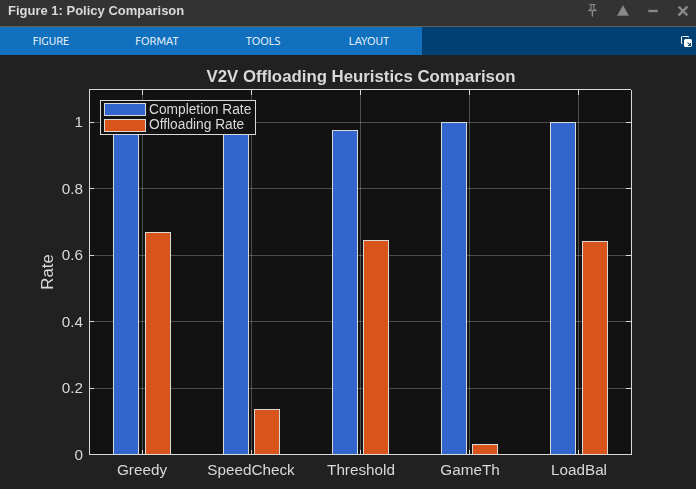
\includegraphics[width=0.48\textwidth]{results.png}
\caption{Completion Rate and Offloading Rate across five V2V offloading heuristics under a 12-vehicle urban intersection scenario with tight AV task deadlines.}
\label{fig:comparison}
\end{figure}
 
\subsection{Overall Task Completion}
A perfect task completion rate of 1.00000 was achieved by Game-Theoretic and Load-Balancing strategies. Speed-Aware Greedy achieved 0.9997, failing on only a small fraction of tasks where mobility conditions marginally violated its link stability filter. Greedy offloading completed 97.47\% of tasks despite having the highest offloading rate of 66.67\%, the aggressive nature of selection exposes tasks to queue buildup and link failures causing missed deadlines. Threshold-Based completed 97.72\% of tasks with an offloading rate of 66.20\%, which shows a similar failure behavior due to the first-fit selection rule accepting service vehicles without assessing queue depth or link duration.
 
\subsection{Effect of Offloading Rate on Reliability}
A relationship is observed between offload aggressiveness and completion reliability. Greedy offloading, has the highest offloading rate of 66.67\% showed the lowest completion rate of 97.47\%. Load-Balancing offloaded 62.90\% of tasks achieved 100\% completion, demonstrating that queue-aware selection even at high volumes prevents missed deadlines. Game-Theoretic and Speed-Aware Greedy stayed conservative, offloading only 1.81\% and 19.83\% of tasks respectively, preferred local execution when the utility gain or speed condition was unsatisfactory. This conservatism eliminated task failures at the cost of leaving available neighbor resources underutilized.
 
\subsection{Mobility and Link Stability}
The low offloading rate of 19.83\% of Speed-Aware Greedy's reflects its strict mobility filter: it only offloads when remote execution time is faster than local processing and within the available service-time window. At urban intersections under high vehicle mobility, this condition is infrequently satisfied, as a result most tasks are handled locally, preventing the link-failure-induced deadline misses observed in the Greedy strategy.
 
\subsection{Energy Efficiency and Fairness}
The utility function of Game-Theoretic strategy penalizes energy cost with a factor $\alpha = 0.2$, resulting in the lowest offloading rate of 1.81\%. It avoided offloading decisions where transmission energy outweighed time saved and achieves 100\% task completion with minimal communication overhead. Load-Balancing achieved the strongest overall balance: it offloaded 62.90\% of tasks by spreading workload across the least-loaded neighbors, preventing queue buildup and sustaining full completion at high task arrival rates.
 
\subsection{Summary of Trade-offs}
The results highlight that no single strategy covered is apt across all dimensions. Greedy offloading maximizes resource utilization but sacrifices reliability under mobility constraints. Game-Theoretic and Speed-Aware Greedy prioritize reliability but does not utilize available neighbor capacity fully. Load-Balancing achieves the best overall balance, combining high offloading volume with perfect task completion by incorporating queue state into its selection logic. These findings suggest that future V2V offloading designs should integrate queue-aware and mobility-sensitive criteria together to sustain performance under realistic urban conditions.
 
\section{Discussion}
The comparison of the five strategies provides several practical observations for designing V2V computation offloading systems. The first finding is that no single method works best in every situation. Greedy offloading reduces delay but performs poorly when vehicles move quickly and tends to use more energy. Similarly, the game-theoretic and load-balancing approaches offer more stable and fair performance, making them better suited for real environments where both resource distribution and link reliability matter.
 
A second key insight is that mobility remains the main factor to limit V2V offloading. Even vehicles with high processing power are unable to contribute effectively if changing speeds reduces the service time available. Strategies that account for relative speed or link duration, such as speed-aware greedy and game-theoretic selection, achieve higher completion reliability as they match tasks to vehicles that will remain in range long enough to meet deadlines.
 
Third, it is observed that task size and communication overhead strongly affect how useful offloading can be. Small tasks are usually completed faster when handled locally. Larger tasks gain from offloading as long as the communication link is stable and excessive delay is not added.
 
Finally, increasing vehicle density creates more offloading opportunities at first, but the benefit does not continue indefinitely. Beyond a certain point, link contention and unpredictable movements reduce overall performance. In these conditions, strategies that spread tasks across multiple vehicles, such as load-balancing, become more effective. Overall, the results show that successful V2V offloading requires balancing delay, mobility, energy use, and queue behavior together.
 
\section{Conclusion}
This study presented a comparative analysis of five heuristic strategies for V2V computation offloading in autonomous vehicular networks. Using realistic mobility traces and a unified simulation framework with 12 vehicles and tight AV task deadlines, we evaluated greedy, speed-aware greedy, threshold-based, game-theoretic, and load-balancing strategies under task arrival rate of 2.0 tasks per second.
 
The findings show that game-theoretic and load-balancing strategies achieve perfect task completion (1.0000) by incorporating energy cost and queue state into offloading decisions. Greedy offloading, despite achieving the highest offloading rate of 66.67\%, yields only 97.47\% completion due to mobility-induced deadline misses. Speed-aware greedy reaches 99.97\% completion through conservative link filtering. Threshold-based selection completes 97.72\% of tasks, limited by its fixed first-fit rule.
 
Vehicle density improves performance up to a moderate threshold before diminishing returns appear due to link contention. Overall, V2V offloading can effectively complement V2I and cloud systems in busy urban intersections, but sustaining performance requires strategies that jointly handle mobility variability, resource fairness, and energy constraints.
 
% \begin{thebibliography}{11}

% \bibitem{chen_delay_v2v}
% C.~Chen \emph{et al.}, ``Delay-Optimized V2V-Based Computation Offloading in Urban Vehicular Edge Computing Networks,'' 
% \emph{IEEE Access}, vol.~8, pp.~18863--18873, 2020.

% \bibitem{hartenstein_vanet_book}
% H.~Hartenstein and K.~Laberteaux, \emph{VANET: Vehicular Applications and Inter-Networking Technologies}. 
% Wiley, 2010.

% \bibitem{chen_vehicular_cloud}
% M.~Chen \emph{et al.}, ``Vehicular cloud computing: A survey,'' 
% \emph{IEEE Trans. on Intelligent Transportation Systems}, vol.~16, no.~3, pp.~1243--1258, 2015.

% \bibitem{mao_mec_survey}
% Y.~Mao, C.~You, J.~Zhang, K.~Huang, and K.~B.~Letaief, ``A survey on mobile edge computing,'' 
% \emph{IEEE Commun. Surveys \& Tutorials}, vol.~19, no.~4, pp.~2322--2358, 2017.

% \bibitem{chen_multiuser_offloading}
% X.~Chen \emph{et al.}, ``Efficient multi-user computation offloading for mobile-edge cloud computing,'' 
% \emph{IEEE/ACM Trans. on Networking}, vol.~24, no.~5, pp.~2795--2808, 2016.

% \bibitem{zhang_energy_efficient_mec}
% K.~Zhang \emph{et al.}, ``Energy-efficient offloading for mobile edge computing in 5G heterogeneous networks,'' 
% \emph{IEEE Access}, vol.~4, pp.~5896--5907, 2016.

% \bibitem{liu_load_balancing_vec}
% J.~Liu, H.~Guo, and H.~Ding, ``Load balancing in vehicular edge computing,'' 
% \emph{IEEE Trans. Vehicular Technology}, vol.~69, no.~3, pp.~2886--2898, 2020.

% \bibitem{bitam_vanet_cloud}
% S.~Bitam, A.~Mellouk, and S.~Zeadally, ``VANET-cloud: A cooperative architecture for mobile cloud computing in VANETs,'' 
% \emph{IEEE Trans. Vehicular Technology}, vol.~64, no.~12, pp.~5447--5459, 2015.

% \bibitem{shladover_cooperative}
% S.~E.~Shladover, ``Cooperative vehicle-highway automation systems,'' 
% \emph{IEEE Trans. Intelligent Transportation Systems}, vol.~12, no.~4, pp.~126--136, 2011.

% \bibitem{abboud_interworking}
% K.~Abboud, H.~A.~Omar, and W.~Zhuang, ``Interworking of DSC-based V2V and cellular LTE-V networks,'' 
% \emph{IEEE Trans. Vehicular Technology}, vol.~65, no.~12, pp.~9457--9470, 2016.

% \bibitem{campolo_modeling_v2v}
% C.~Campolo, A.~Molinaro, and A.~O.~Berthet, ``Modeling V2V communications for cooperative awareness,'' 
% \emph{IEEE Commun. Magazine}, vol.~55, no.~8, pp.~80--86, 2017.

% \end{thebibliography}

\bibliography{biblio}
\bibliographystyle{IEEEtran} 

\end{document}
 



